%----------------------------------------------------------------------------
\section{Arclenyomatok adatvédelmi elemzése}
\label{sec:4}

%--------------------------------------------------------------------------------------------------
\subsection{Támadó modellezése}  % 1 oldal
% - Támadómodell bemutatás (copy ábra Gábortól, lényeget leír)
% - Jelenlegi arcfelismerő rendszerek sebezhetősége, hogyan férhet hozzá
% - Feltételezzük, hogy a támadó interneten elérhető datasetekhez hozzájut ami alapján betanít classifiert és ezt használva tud kinyerni adatot. Következő fejezetben erre mutatunk példát hogyan lehetséges

A következőkben az arcfelismerő rendszerek sebezhetőségét fogom elemezni. Az arcfelismerő rendszerek általános működését a [REF] fejezetben korábban bemutattam. Az adatvédelmi elemzéshez szükséges definiálnom egy támadó modellt. Tegyük fel, hogy egy cégnél alkalmaznak arcfelismerő rendszert a dolgozók azonosítására. Az épület számos helyisége be le van fedve CCTV térfigyelő kamerákkal, amelyek egy központi arcfelismerő rendszernek továbbítják a felvételeket. Új dolgozó regisztrációja során az arcfelismerő rendszer néhány felvétel alapján kiszámolja a dolgozó arcát lebjobban leíró arclenyomatát, amit egy központi szerveren tárol. Miután a dolgozó arclenyomata szerepel az adatbázisban, a térfigyelő kamera felvételek alapján lehetséges őt azonosítani. Egy ilyen arcfelismerő rendszernek a főbb részei: 

% TODO ide lehet szoftver példákat hozni ha kell content
% magyar szavakat kéne használni
\begin{enumerate}
	\item Kamera rendszer: amely a nyers képkockákat továbbítja az adatfeldolgozó egységnek
	\item Feature extractor: amely az egyes kékkockákon végzi a gyorsan lefuttatható arcdetektálást. Ha sikeresen talál emberi arcot az egyik kékkockán, arra elvégzi az arc geometriai transzformációját, majd az arcból kinyeri az arclenyomatot.
	\item Adatbázis: Az ismert, címkézett arclenyomatok tárolására szolgál.
	\item Matcher: A kinyert arclenyomatot összehasonlítja az adatbázisban tárolt dolgozók arclenyomataival, majd azokon valamilyen távolság (pl: Euklideszi távolság) metrika alapján megállapítja a legvalószínűbb találatot. Ha a legkisebb távolság egy bizonyos küszöbértéknél kisebb, akkor a dolgozót sikeresen azonosította, ellentkező esetben ismeretlen személynek nyilvánítja.
\end{enumerate}

Míg az ilyen arcfelismerő rendszer több módon is támadható, a dolgozatom során azzal az esettel foglalkozom, hogy a rosszindulatú fél valamilyen módon hozzáférést nyer az arclenyomat adathalmazhoz, ami lehet egy belső alkalmazott aki kiszivárogtatja az adatbázist, vagy akár egy külső támadó, például hacker aki sikeresen feltöri rendszert. Előfordulhat, hogy a támadó az adatbázisnak egy kisebb részéhez fér hozzá, de dolgozatom során a legerősebb támadót feltételezem, aki a teljes adatbázishoz hozzáfér, illetve feltételezem, hogy az arclenyomatok titkosítás nélkül vannak tárolva a szerveren.

% TODO saját ábra?
\begin{figure}[ht]
	\centering
	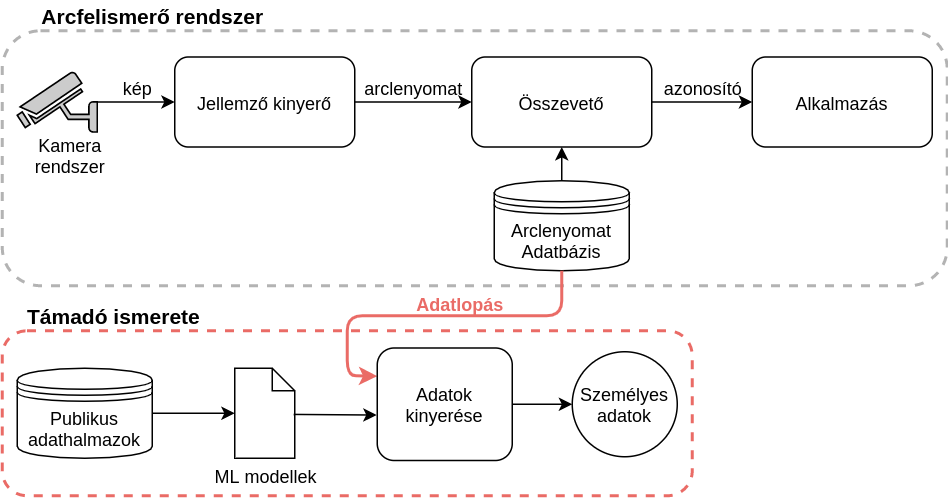
\includegraphics[width=1\columnwidth]{figures/attacker_model.png}
	\caption{ideiglenes ábra}
	\label{fig:attacker}
\end{figure}

A támadó modellezését a \ref{fig:attacker}. ábra mutatja be. Miután a támadó valamilyen módon hozzáférést szerzett a központi szerverhez, amin az arclenyomatok vannak tárolva, elképzelhető, hogy képes lesz az arclenyomatokból személyes adatokat kinyerni az adatalanyokról. Személyes adatnak minősül bármilyen adat, ha közvetlenül beazonosítható általa az érintett személy (közvetlen azonosítók), vagy ha közvetetten (kvázi-azonosítók) \cite{GDPR2018}. Személyes adat lehet például a személy demográfiai adatai, mint például a személy életkora, a neme, vagy a rassza. 

Feltételezhetjük, hogy a támadó a személyes adatok kinyeréséhez egy saját fejlesztésű algoritmust használ, ami lehet például egy gépi tanulási modell is. Ha a támadó képes megfelelően nagy valószínűséggel, megbízható módon kinyerni a személyes adatokat, akkor a támadó feltételezheti, hogy a kinyert adatok valósak. A sikeresen kinyert adatokat majd saját célból fel tudja használni a támadó, például újraazonosításos támadáshoz. A személyes adatok kiszivárgásának adatvédelmi kockázatait a \ref{sec:adatvedelmi_elemz}. fejezetben fejtem ki bővebben.

A kérdés az, hogy milyen eljárással lehetséges egy arclenyomatból kinyerni az adatalan érzékeny információit? A munkám során erre a kérdésre kerestem választ. Feltételezésem az volt, hogy az interneten ingyenesen, publikusan elérhető emberi arcokról készült fotókból összeállítható egy nagy méretű adathalmaz, amihez rendelkezésre állnak a fotón látható valamennyi személy demográfiai adatai, például a pontos vagy becsült életkora, neme és rassza, vagy bármilyen adat ami fotó alapján ember által megadható, és később segíthet az illető azonosításában. Ha sikerül egy ilyen adathalmazt összeállítani, akkor az arcképek alapján az arcfelismerő rendszer működéséhez hasonlóan minden arcképről generálhatunk arclenyomatokat. Ezt követően rendelkezünk az arclenyomatokkal, és a hozzájuk tartozó címkékkel.

Miután megvan az arclenyomat adathalmaz, az alapján képesek vagyunk betanítani egy gépi tanulási modellt, ami az arclenyomatok és a hozzájuk tartozó címkék alapján képes tanulni. A betanítás után a modell használható arra, hogy új, nem látott arclenyomat mintákra becslést adjon. Visszatérve a támadóhoz, ha a támadó rendelkezik egy előre betanított gépi tanulási modellel, azt felhasználhatjra arra, hogy a szerverről szerzett arclenyomat adatbázisból érzékeny adatokat nyerjen ki. 

A támadó sikerességének feltétele az, hogy képes hozzáférni a szerveren tárolt arclenyomatokhoz, illetve az, hogy a gépi tanulási modellje milyen megbízhatósággal képes becslést hozni a személyes adatokra. A két feltétel közül a másodikkal foglalkozom a továbbiakban. Azt vizsgáltam, hogy modern tanuló algoritmusokkal milyen eredmény érhető el.

%--------------------------------------------------------------------------------------------------
\subsection{Adathalmazok}  % 3-4 oldal

Első lépésként szükségem volt egy megfelelően felcímkézett arclenyomat adathalmazra. Ezt az adathalmazt használom fel arra, hogy az alapján tanítsak be gépi tanulási modelleket, amelyek majd képesek becslést adni személyes adatokra. Egy-egy modell csak egy személyes adatra tud becslést adni, ezért több modellre van szükség. Célom az volt, hogy személyes adatok közül az illető életkorát, nemét és rasszát becsüljem meg. Ehhez szükséges tanító mintakészlet, amiben az életkor, nem és rassz meg van címkézve. Elvárás volt még az is, az arclenyomat adathalmazban minden személynek saját azonosító címkéje legyen, illetve lehetőleg minél több arclenyomat tartozzon egy-egy személyhez. Erre azért van szükség, mert az arclenyomatokon vizsgáltam az identifikációs modell teljesítőképességét is. 

Mivel a feladatból adódóan az adathalmazzal szemben támasztott elvárások eléggé specifikusak, ezért szükség volt saját adathalmaz létrehozására. Azért, hogy meggyorsítsam a munkámat, kiindulásnak kerestem olyan online elérhető, arcképeket tartalmazó adathalmazt, ami már előre fel van címkézve. Ha létezik egy megflelő arckép adathalmaz, akkor a képekből egyessével kinyerhetőek az arclenyomat vektorok. 

Az arckép adathalmazzal szemben az elvárások a következők:
\begin{itemize}
	\item Lehetőleg kutatási célra lettek létrehozva, az enyémhez hasonló feladatra. Ennek megfelelően az arcképek már előre vannak készítve a feldolgozáshoz (pl. arc kivágása a képből).
	\item Az adathalmaznak megfelelően nagynak kell lennie ahhoz, hogy gépi tanulási modellt sikeresen be lehessen tanítani róla.
	\item Egy emberről lehetőleg minél több kép legyen ahhoz, hogy a generált arclenyomatok alapján identifikáció jól működjön. Minél több képünk van egy illetőről, anál biztosabban lehet meghatározni az ember arcát legjobban leíró arclenyomatot.
	\item A képek megfelelő demográfiai adatokkal vannak címkézve. Esetemben a szükséges címkék: az életkor, nem és a rassz.
\end{itemize}

Nehéz olyan adathalmazt találni, amiben mindhárom számunkra fontos demográfiai adat szerepel. Több arckép adathalmaz jónak tűnt elsőre, de az elvárások közül nem felelt meg egynek. Néhány ilyen adathalmaz amivel foglalkoztam: Labled Faces in the Wild \cite{labledfacesinthewild2008}, Face Image Project \cite{faceimageproject2014}, CelebA \cite{celebA2015}. A FairFace \cite{fairface2021} egy viszonylag új adathalmaz, ami nagyon igéretesnek tűnt, mert mindhárom demográfiai adatot tartalmazza, és az egyes osztályok aránya kiegyensúlyozott, viszont nem tartalmaz identifikációs címkét.

Végül nem sikerült olyan adathalmazt találnom ami minden kritériumnak megfelel, ezért két külön adathalmazt használtam fel. Az egyik a VGGFace2 \cite{vggface22018} amit rassz és nem becslésére használtam fel, a másik pedig az IMDB-WIKI dataset \cite{imdbwiki2018}, amit életkor becsléshez használtam fel. A két választott arckép adathalmazt szükség volt feldolgozni ahhoz, hogy azokból gépi tanulási modellt lehessen tanítani. A feldolgozás menetét mutatom be a következő részekben.

\subsubsection*{VGGFace2 adathalmaz}
% TODO ha van idő -> újragenerálni az ábrákat a gábor adathalmazára (szűrés utáni) mert abban nem 540 000 embedding van hanem csak 70k v mennyi.

Jelenleg az egyik legnagyobb publikusan elérhető, kutatási célra készült arckép adathalmaz a VGGFace2. Az adathalmaz 3,31 millió arcképet tartalmaz mindössze 9131 emberről, átlagosan 362,6 kép mindenkiről. A képeket a Google képkeresőjével gyűjtötték össze. Az adathalmaz képein sokféle ember szerepel, eltérő demográfiai adatokkal és eltérő szakmával (pl. vannak színészek, sportolók, politikusok). A képeken látható emberek többféle pózban láthatóak, sokféle megvilágításban. Az összegyűjtött képeket automatikusan és manuálisan is szűrték.

A VGGFace2 alapból nem tartalmaz rassz címkéket, viszont a Salernói Egyetem MIVIA kutatócsoportja manuálisan felcímkézte az adathalmazt rassz címkékkel, és a munkájukat publikusan elérhetővé tették VMER névvel \cite{vmer2020}. A VMER-rel kiegészítve a VGGFace2 címkéit, így már van rassz, nem és identifikációs címke is az összes mintához.

Az arcképeket egyesével dolgozza fel egy script, ami az arcképekből kinyeri az arclenyomatokat. Ehhez a face\_recognition Python könyvtárat \cite{face_recognition} használtam fel, ami a [REF sec:problema]. fejezetben taglalt módon találja meg, és alakítja át a képen látható arcokat arclenyomattá. Az arclenyomatok kinyeréséhez a dlib-et \cite{dlib2009} használja, így a kapott arclenyomatok 128 dimenziós lebegőpontos vektorok lesznek. Az adathalmazban előfordulnak olyan képek, ahol több ember arca is látható, (például a háttérben elsétál valaki). Ez problémás, mivel ilyenkor nem egyértelmű, hogy a képen látható melyik archoz tartozik az annotáció. E miatt a scriptem csak olyan képekkel foglalkozott, ahol pontosan egy arcot sikerült azonosítani. A script-ből egy függvény látható a \ref{lst:get_encoding}. kódrészleten.

\begin{lstlisting}[language=python, caption={Arclenyomat vektorok kinyerése.}, label=lst:get_encoding]
def get_encoding(filepath):
  # kep beolvasasa
  image = face_recognition.load_image_file(filepath) 
  # arcok detektalasa 
  face_locations = face_recognition.face_locations(image,
    number_of_times_to_upsample=1, model="cnn")
  if (len(face_locations) == 1): 
    # arclenyomat vektor
    return np.array(face_recognition.face_encodings(image,face_locations))[1]
  return None
\end{lstlisting}


Mivel 3,3 millió arcképet kellett feldolgozni, a Python scriptet Google Colab-en futtattam, aminek az az előnye, hogy ingyenesen lehet használni korszerű GPU-kat, illetve az adathalmaz feldarabolásával párhuzamosan több session-t is lehet futtatni, jelentősen felgyorsítja a képek feldolgozását.

A következő lépés az adathalmaz tisztisása volt, azaz kiszűrni azokat a képeket, amelyek valamilyen okból rossz minőségűek (például távoli fotó, rossz fényviszony vagy fura szögből készült a kép), vagy az illető a többi képhez képest nagyon eltérően néz ki. Az arclenyomatok szűréséhez minden személyhez kiszámítottam az átlagos arclenyomatot (centroid), és a centroidtól vett távolság alapján a túl nagy távolságra lévő arclenyomatokat szűrtem az adathalmazból. 

A feldolgozás és szűrés után kapott adathalmaz közel 3 millió arclenyomatot tartalmaz. Minden arclenyomathoz tartozik egy ID címke ami azonosítja az képen látható személyt. Egy ID-hoz legalább 50 arclenyomat tartozik. E mellett van még nem címke (férfi, nő), és rassz címke (African American, East Asian, Caucasian Latin, Asian Indian). Ekkor probléma volt az, hogy az egyes osztályokhoz sokkal több minta tartozott mint más osztályokhoz. A leggyakoribb a fehér férfiak aránya volt, míg a legritkább az afroamerikai nők. Az osztályok arányát a \ref{fig:vgg_imba}. ábra mutatja be.

\begin{figure}[ht]
	\centering
	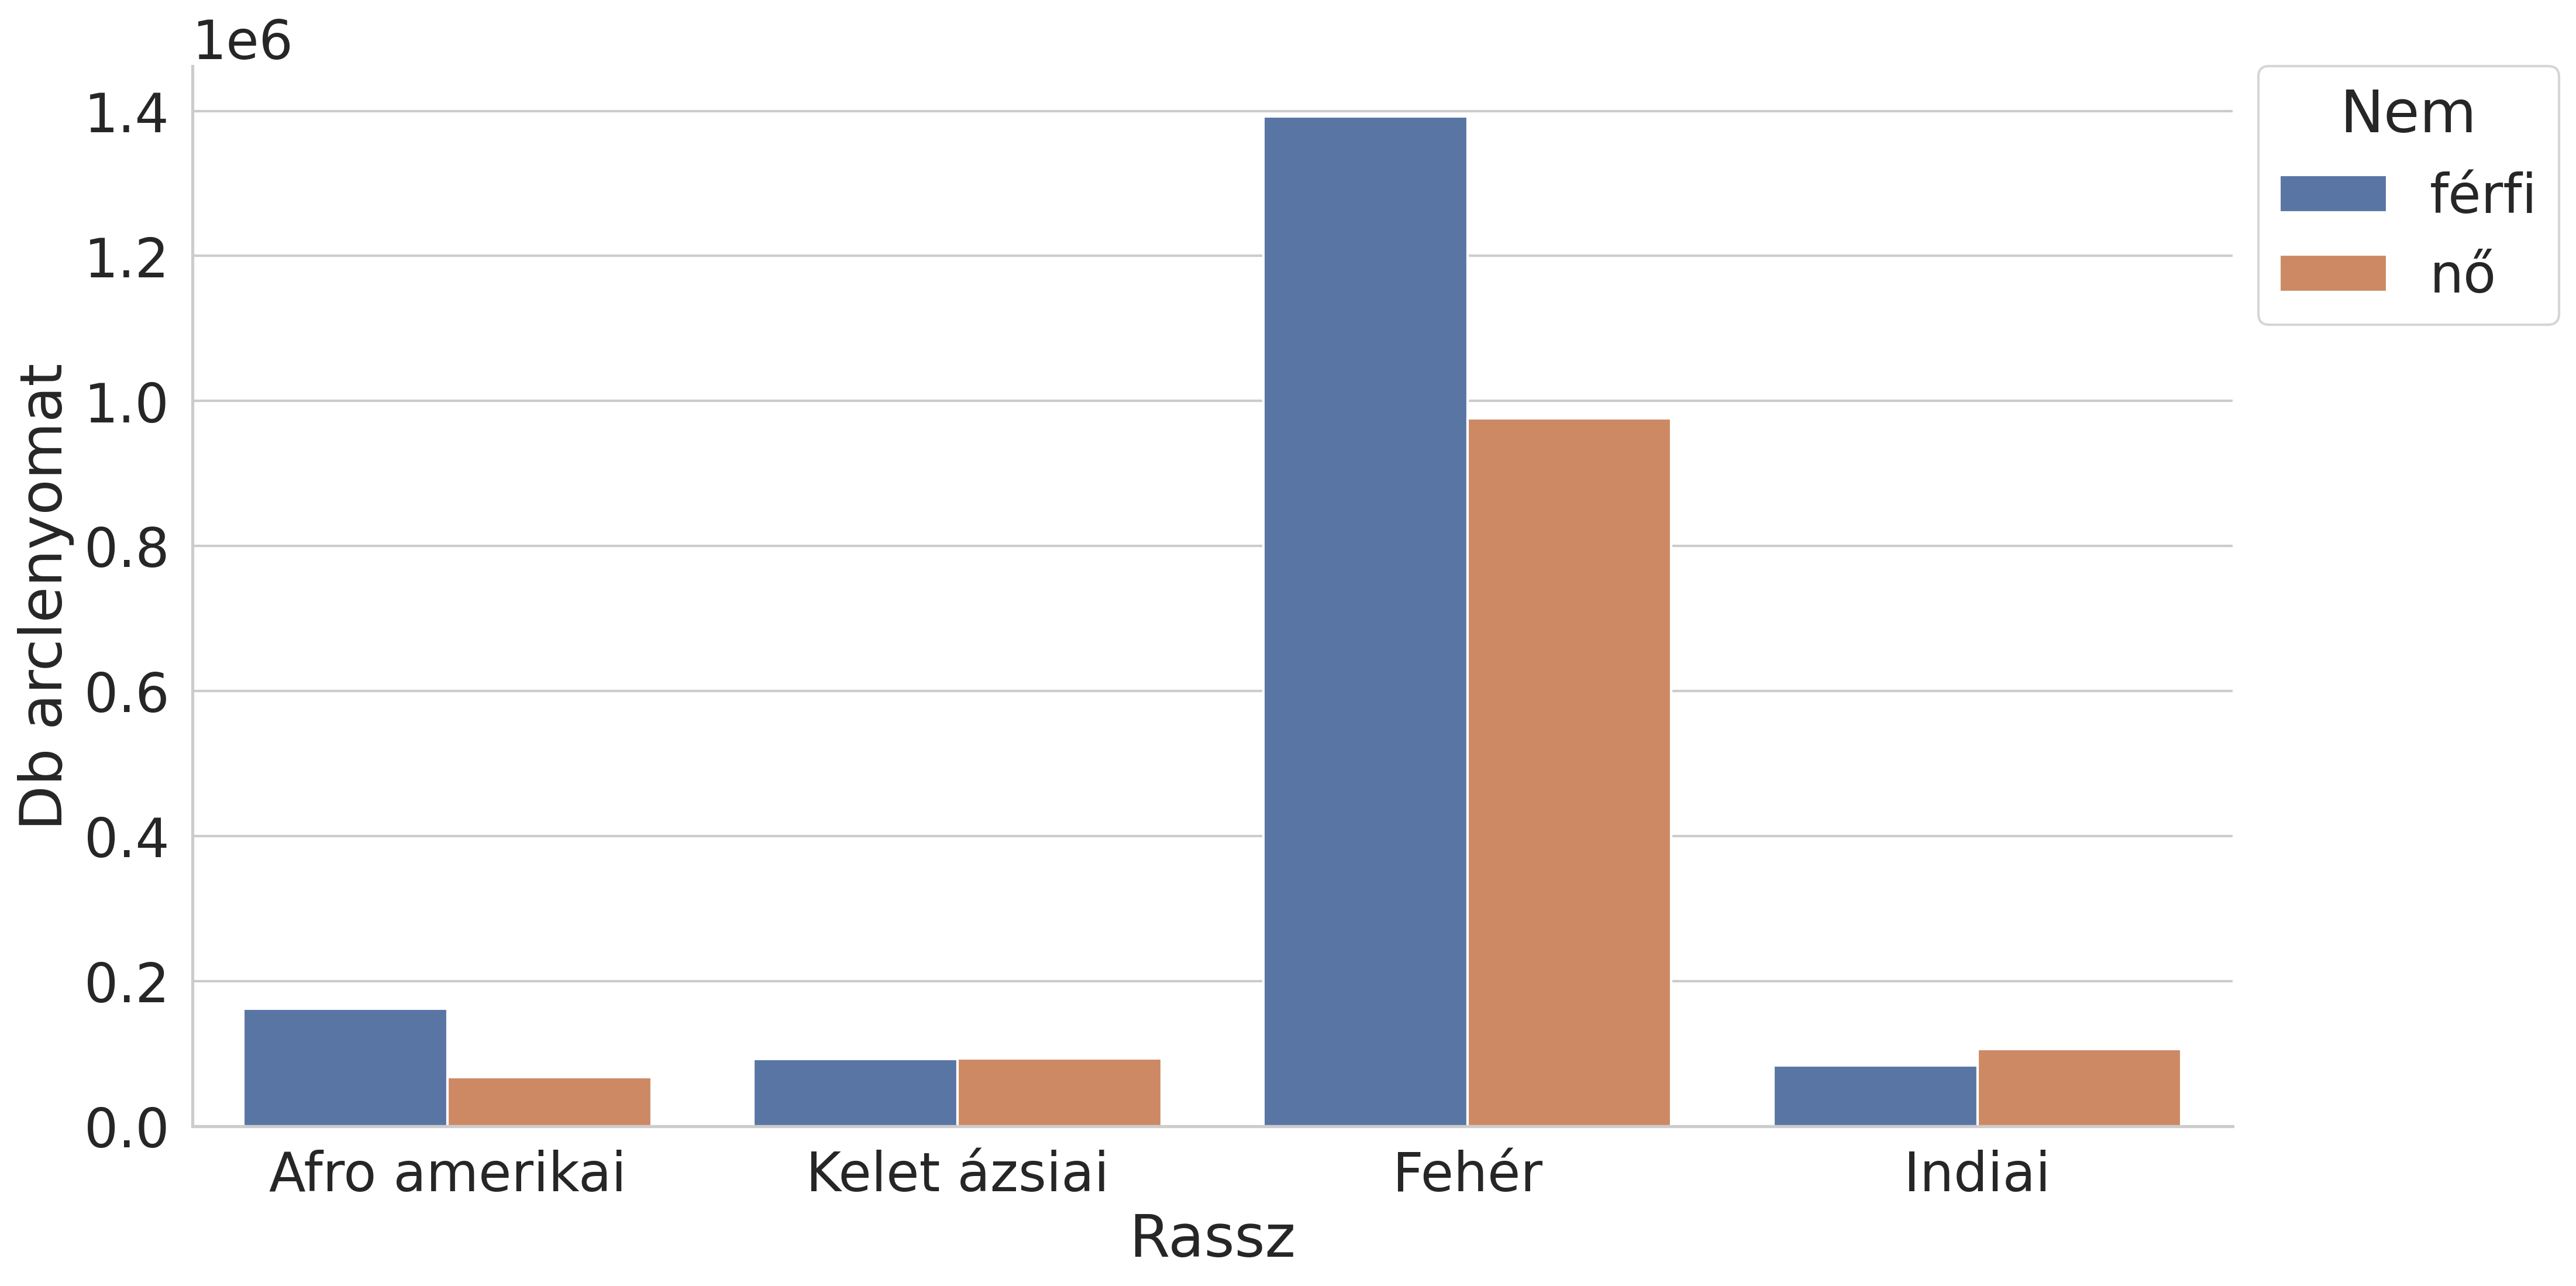
\includegraphics[width=1\columnwidth]{figures/VGG_imba.png}
	\caption{Osztályok aránya az arclenyomat adathalmazban.}
	\label{fig:vgg_imba}
\end{figure}

Az osztályok eloszlásának aránytalansága problémát jelent az osztályozó modellek tanításakor, ezért szükséges volt az adathalmazt kiegyensúlyozni. Az adathalmaz kiegyensúlyozása minták eltávolításával érhető el. Legkevesebb kép az afroamerikai nőkről van az adathalmazban, ezért ehhez mérten szűkítettem a többi csoportot. Az embeddingek kivételénél fontos volt, hogy továbbra is legalább 50 kép maradjon minden személyről, ezért nem véletlenszerűen vettem ki a képeket, hanem ID-k alapján csoportosítva. Az egyes demográfiai csoportoknál kilistáztam az oda tartozó ID-kat, és egyes ID-khoz tartozó képek számát. Az ID-kat képszám szerint csökkenő sorrendben távolítottam el, amíg a csoport meg nem közelítette a szükséges méretet. Ezzel a módszerrel sikerült elérni, hogy minden rassz-nem párhoz ugyanannyi ember tartozott. A kiegyensúlyozott után az osztályok eloszlása a \ref{fig:vgg_ba}. ábrán látható.

\begin{figure}[ht]
	\centering
	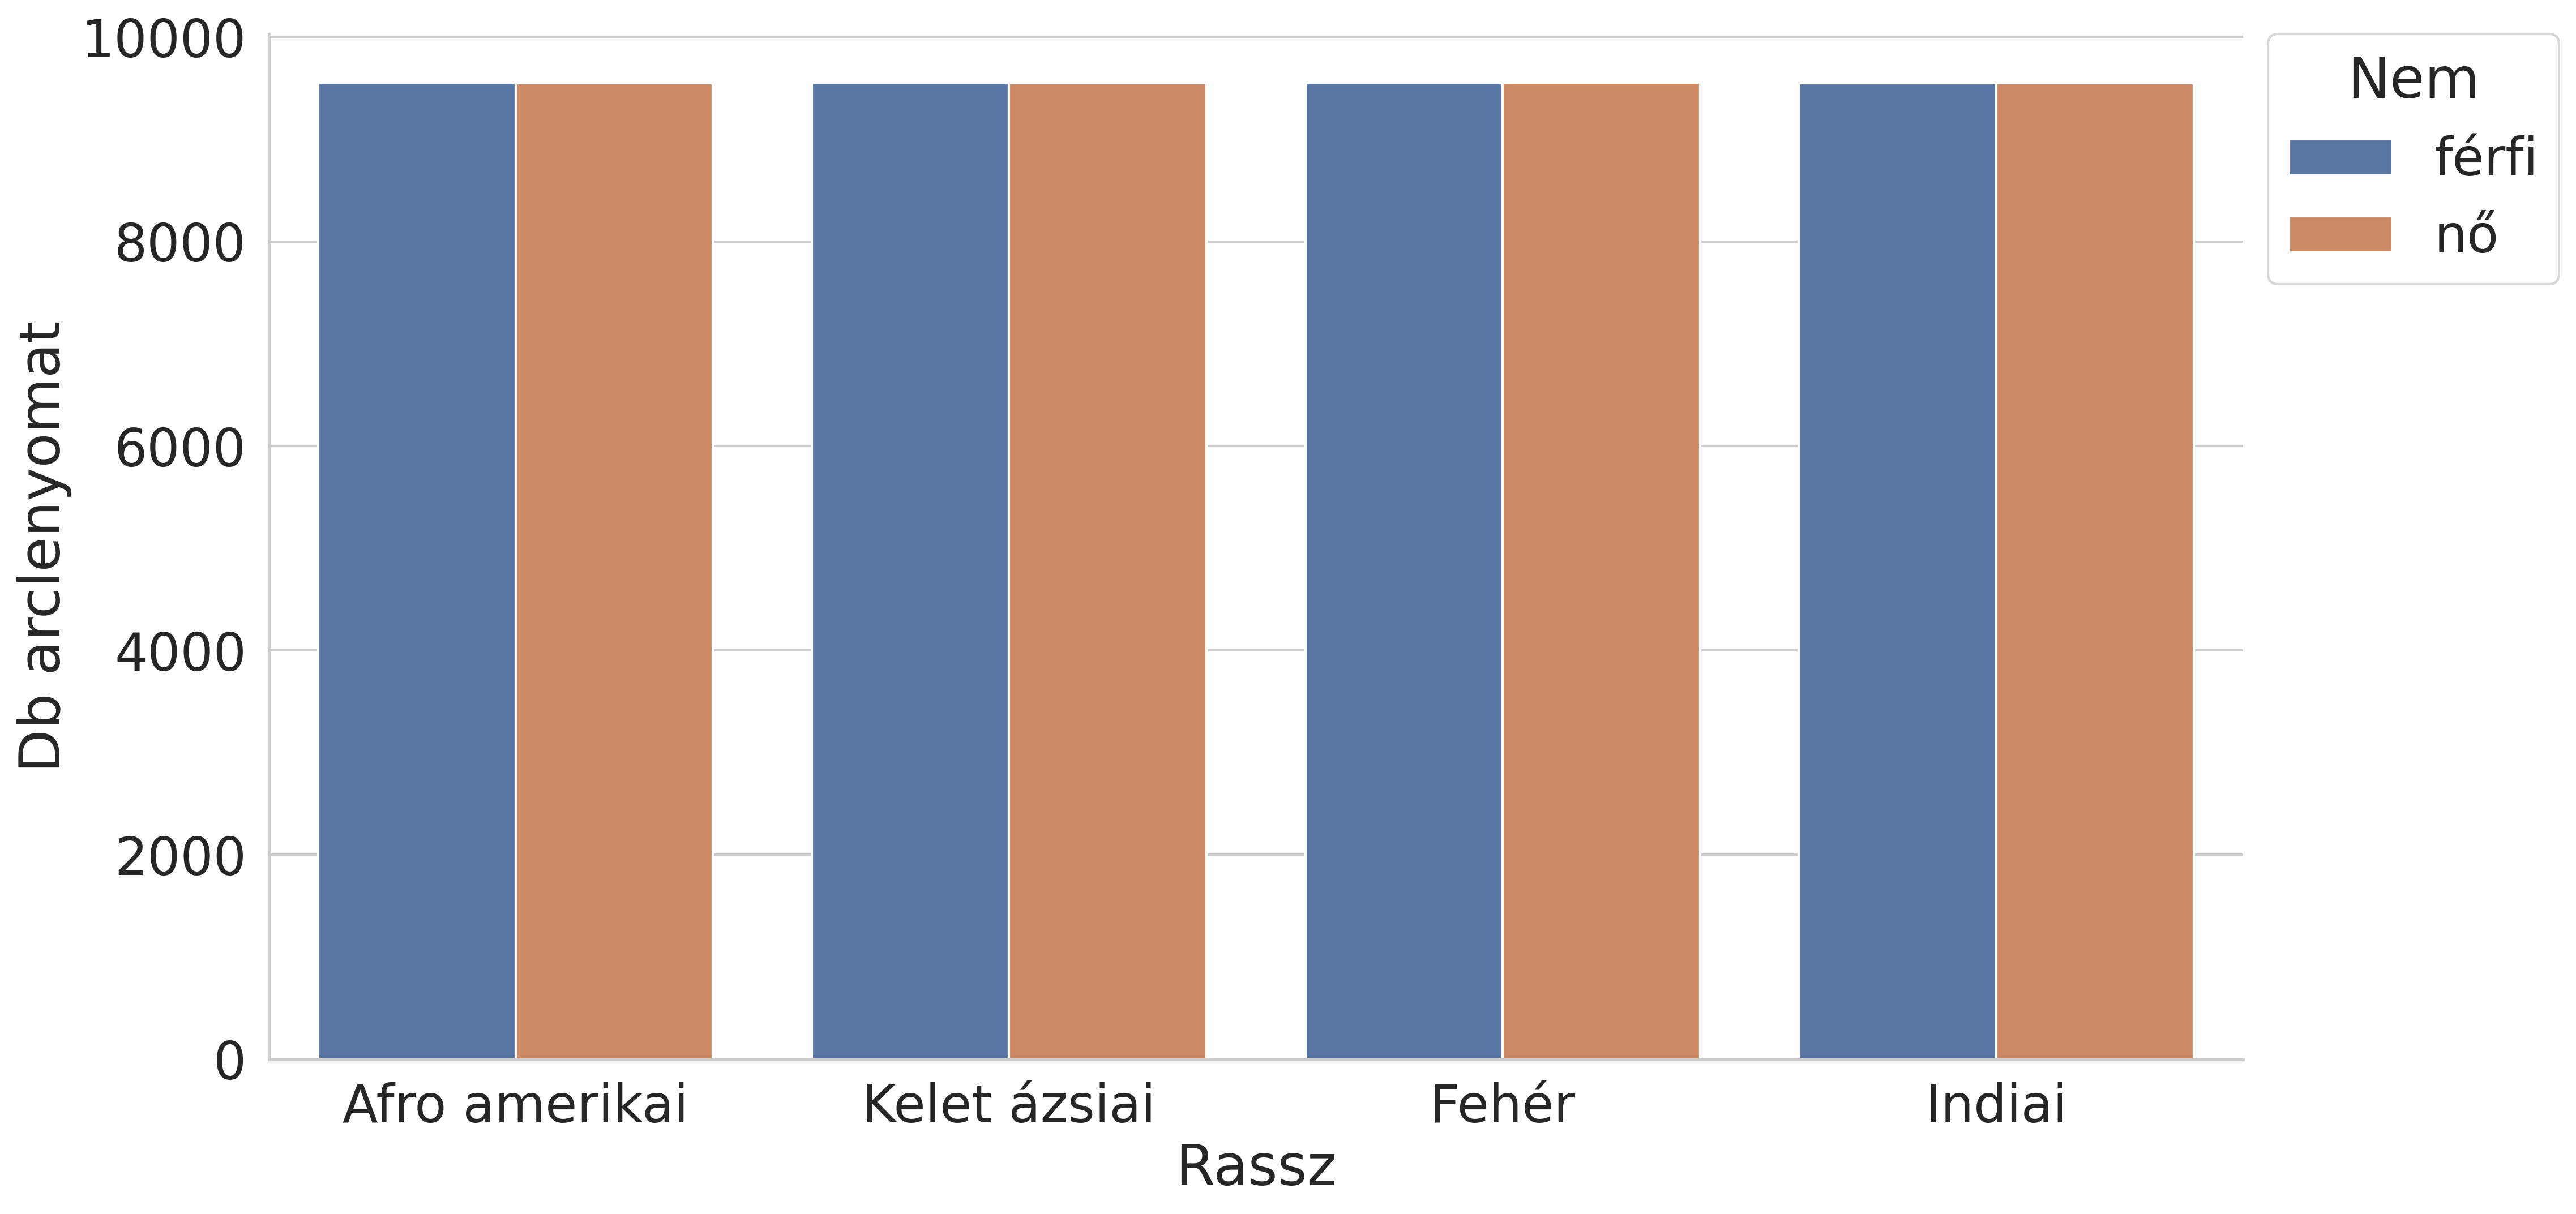
\includegraphics[width=1\columnwidth]{figures/VGG_balanced.png}
	\caption{Osztályok aránya az kiegyensúlyozás után.}
	\label{fig:vgg_ba}
\end{figure}

Az eredeti 3,3 millió képből végül 540000 arclenyomat készült, ami továbbra is nagy adathalmaznak tekinthető. Ez elegendően nagy ahhoz, hogy ez alapján osztályozó modelleket lehessen rajtuk betanítani.

\subsubsection*{IMDB-WIKI adathalmaz}

Mivel a VGGFace2 adathalmaz nem tartalmaz életkor címkét, ezért tovább folytattam a keresést. Választásom az IMDB-WIKI \cite{imdbwiki2018} adathalmazra esett. Ez az egyik legnagyobb, nyilvánosan elérhető arckép adathalmaz, ami tartalmaz azonosító címkét, nemet és életkort is. Az adathalmaz két részből áll: IMDB filmekről és filmszínészekből álló adatbázisból kinyert fotókból, illetve a Wikipédiáról szerzett fotókból. Sajnos a Wikipédiáról szerzett képekhez nem tartozik azonosító címke, így csak az IMDB-ről szerzett fotókat használtam fel.

Az IMDB-WIKI adathalmaz képekből, és hozzájuk tartozó címkékből áll. A címkék egy metadata fileban találhatóak, ami többek között tartalmazza a képen látható személy nevét, nemét, a születési dátumát, illetve azt, hogy mikor készült a fotó. A életkort a képen látható személy születési dátumából, és a kép keletkezésének dátuma alapján lehet kiszámolni. A képek jelentős része csoportkép, azaz több arc is látható rajtuk. A képek közül csak azokat használtam fel, ahol pontosan egy arcot lehetett detektálni. Továbbá, kiválasztottam azokat az azonosítókat, amihez legalább 30 fotó tartozik.

A weboldalról letölthetőek az eredeti, teljes méretű képek, illetve a már megvágott csak arcokat tartalmazó képek is. A képeken az arcok középre vannak rendezve 40\%-os ráhagyással. A képek feldolgozásánál ezért levágtam ezt a 40\%-ot, így gyorsabb a feldolgozás és jelentősen több képen sikerült arcot detektálni. Az arcokhoz tartozó képeket a VGGFace2-nél bemutatott módszerrel alakítottam át arclenyomat vektorokká.

\begin{figure}[ht]
     \centering
     \begin{subfigure}[b]{0.45\columnwidth}
         \centering
         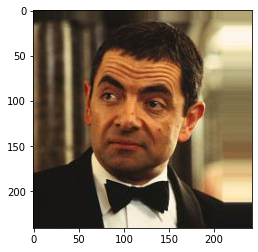
\includegraphics[width=1\columnwidth]{figures/mrbean.png}
     \end{subfigure}
     \begin{subfigure}[b]{0.45\columnwidth}
         \centering
         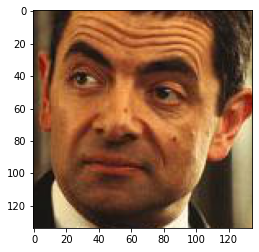
\includegraphics[width=1\columnwidth]{figures/mrbean_crop.png}
     \end{subfigure}
        \caption{Az eredeti és a megvágott kép}
\end{figure}


Az adathalmaz képeit vizsgálva azt tapasztaltam, hogy néhány fotón nem a címkének megfelelő személy szerepelt. A hibásan címkézett képek kiszűréséhez a már feldolgozott arclenyomat vektorokat használtam fel. Egy személyhez tartozó arclenyomat vektorok alapján kiszámítottam a vektorok súlypontját (centroidját), és ehhez mért Euklideszi távolságok alapján szűrtem ki a kiugró értékeket. Azt a határt, ami alatt elfogadta az arclenyomat vektor értékét 0,5-re állítottam be, ami viszonylag szigorúnak számít. Ezt az eljárást szemlélteti a \ref{lst:cent}. kódrészlet.

% TODO itt kicsit gebasz van a page break miatt
% \noindent
% \begin{minipage}{\columnwidth}
\begin{lstlisting}[language=python, caption={Arclenyomatok szűrése távolság alapján.}, label=lst:cent]
def filter(df, cutoff=0.5):
	encodings = df.iloc[:,4:].values  # egy szem(*@\color{codegreen}é@*)lyhez tartoz(*@\color{codegreen}ó@*) arclenyomatok
	centroid = np.mean(encodings, axis=0)  # s(*@\color{codegreen}ú@*)lypont sz(*@\color{codegreen}á@*)m(*@\color{codegreen}í@*)t(*@\color{codegreen}á@*)s
	distance = np.linalg.norm(encodings - centroid, axis=1)  # euklideszi t(*@\color{codegreen}á@*)vols(*@\color{codegreen}á@*)g
	return df.index[distance > cutoff]
\end{lstlisting}
% \end{minipage}

Feldolgozás után közel 90000 arclenyomat vektort kaptunk eredményül. Az adathalmazon belül a nemek aránya közel azonos, viszont az életkor eloszlása már kevésbé egyenletes (lásd: \ref{fig:agedist}. ábra). Mivel a képek az IMDB weboldalról lettek összegyűjtve, ezért főleg színészekről, filmrendezőkről vannak képek, akik tipikusan a 20-40-es életkor tartományba esnek. E miatt kiskorúakról és idős emberekről viszonylag kevés kép van az adathalmazban.

\begin{figure}[ht]
	\centering
	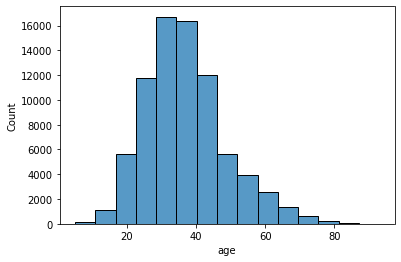
\includegraphics[width=0.7\columnwidth]{figures/IMDB_age_dist.png}
	\caption{IMDB adathalmazban az életkor eloszlása.}
	\label{fig:agedist}
\end{figure}

%--------------------------------------------------------------------------------------------------
\subsection{Modellek betanítása, eredmények}  % 1 oldal RFC, 1-2 oldl eredmények
% - RFCről röviden, miért ezt választottam, 
% - Tanítás módszeréről (használt paraméterek, modell jellemzők, age hogy lett kezelve, ID hogy lett kezelve) 
% - Betanított modellek accuracy precision, recall, F1 score, Confusion matrix, ROC curve

% mi az az RFC, röviden

Az elkészült arclenyomat adathalmazok alapján betaníthaunk valamilyen osztályozó tanuló algoritmust, ami az arclenyomatok alapján becslést tud adni a személy demográfiai adataira. Gyakorlatban ehhez három osztályozó modellt tanítottam be: egyet a nem predikcióhoz, egyet a rasszhoz, egyet az életkorhoz. E mellett készítettem egy identifikációs modellt is, ami az arclenyomatok alapján azonosítani tudja a személyt. A három osztályozó modellhez döntési erdő struktúrát használtam.

Az egyik legalapvetőbb osztályozási algoritmus a döntési fa (angol szakirodalomban decision tree). A döntési fa tanítása során a tanító halmazt lépésenként két halmazra bontja szét az adatok különböző jellemzőire teljesülő vagy nem teljesülő feltétel alapján. Ezt a szétválasztó lépést majd sokszor megismétli, minden lépésnél egy-egy elágazást hoz létre. A feltételek alapján szétválogatott adatok így különböző osztályokba kerülnek. A döntési fák általánosítási képessége javítható, ha azokat egy szakértő együttes (ensemble) struktúrába rendezzük. Ekkor a tanító mintakészletre több, eltérően inicializált döntési fát tanítunk be, amik együttesen egy ``döntési erdőt'' képeznek. Ekkora egy bemeneti mintára a döntési erdő minden fája képez egy becslést, hogy melyik osztályba tartozik a minta. Az döntési erdő kimenete az az osztály lesz, amelyikre a legtöbb döntési fa szavazott. Az osztályozó modellekhez a Scikit-learn Python könyvtár döntési fa implementációját használtam. Ennek a modellnek az az előnye, hogy a használata egyszerű, mivel hiperparaméterek rögzítése nélkül is jó eredményeket lehet elérni.

\subsubsection*{Nem becslése}

A nem becslő osztályozó modell tanításához a VGGFace2 arclenyomat adathalmazt használtam fel. Az arclenyomatok $N\times128$ dimenziós mátrix formában vannak, a hozzájuk tartozó címkék $N\times1$ méretű vektorban, ahol $N$ az adathalmaz mintáinak száma. A teljes mintakészletet felosztottam tanító halmazra és teszt halmazra úgy, hogy a tanító halmaz a minták 70\%-át, a teszt halmaz a minták 30\%-át tartalmazza. A minták osztályozásához 100 döntési fábób álló véletlen erdő modellt használtam. A modell betanítása után a pontosságát a teszt adathalmazon ellenőriztem. A teszt halmaz kb 23000 mintából állt, amiből a modell csak 276 mintánál tévesztett. A modell jóságát a \ref{fig:conf_sex}. ábra mutatja, ahol az osztályozó igazságmátrixa látható. 
\begin{figure}[ht]
	\centering
	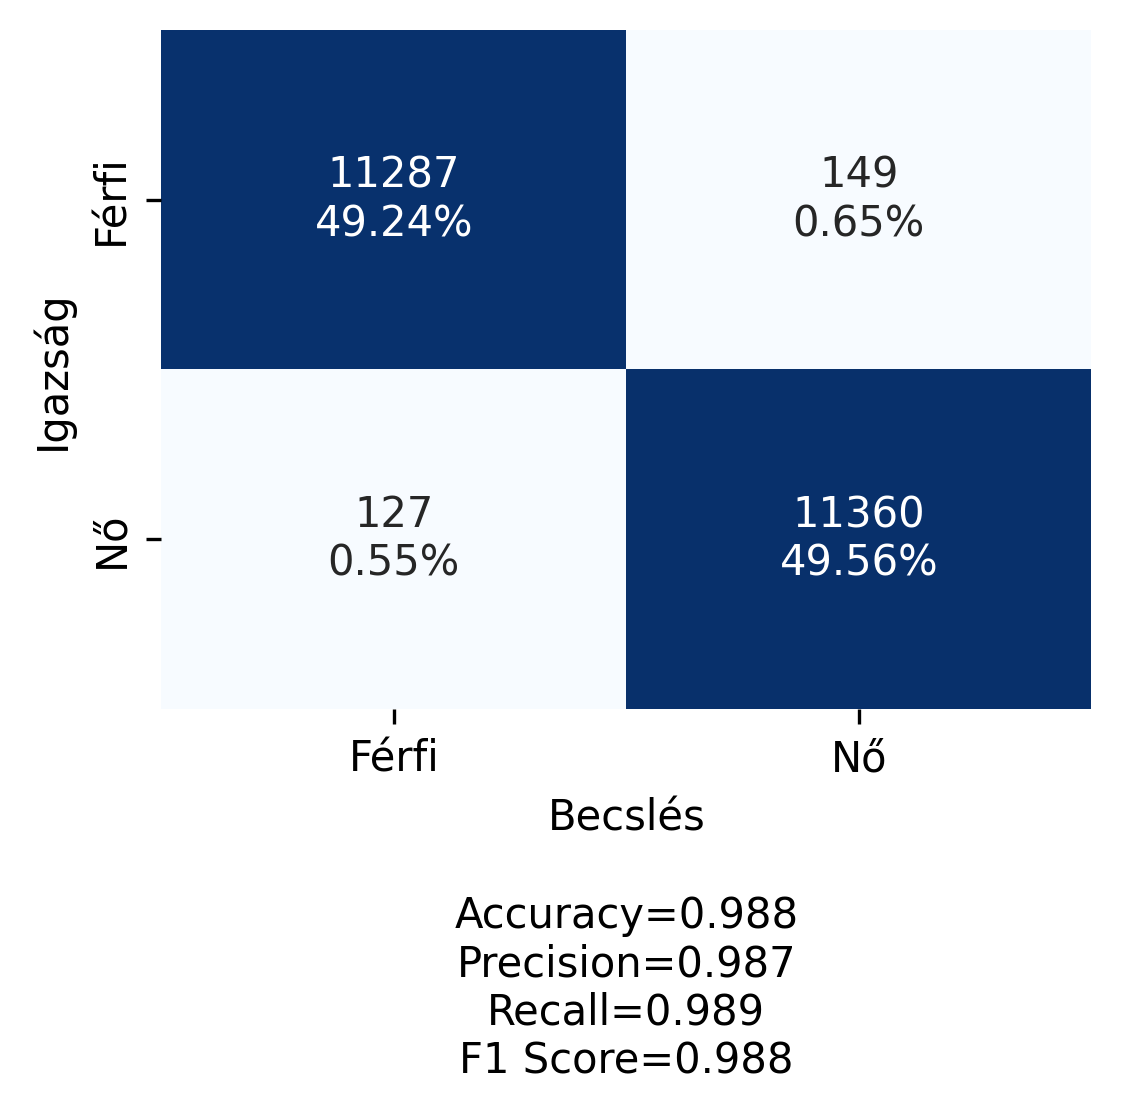
\includegraphics[width=0.55\columnwidth]{figures/conf_sex.png}
	\caption{A nemet osztályozó modell igazságmátrixa és pontossági metrikái.}
	\label{fig:conf_sex}
\end{figure}

\subsubsection*{Rassz becslése}
A rassz osztályozó modellt a nem osztályozóhoz hasonlóan tanítottam be, azzal a külömbséggel, hogy itt bináris osztályozás helyett már 4 osztályunk van, ami nehezebb feladatnak számít. A négy osztály: afro amerikaiak, kelet ázsiaiak, fehérek, és indiaiak. A VGGFace2 adathalmaz kiegyensúlyozottságának köszönhetően itt is sikerült jó pontosságot elérni. A modell igazságmátrixát a \ref{fig:conf_race}. ábra mutatja be. A többosztályos osztályozó modell pontossági metrikáinak kiszámításához ``macro'' átlagoló módszert használtam.

\begin{figure}[ht]
	\centering
	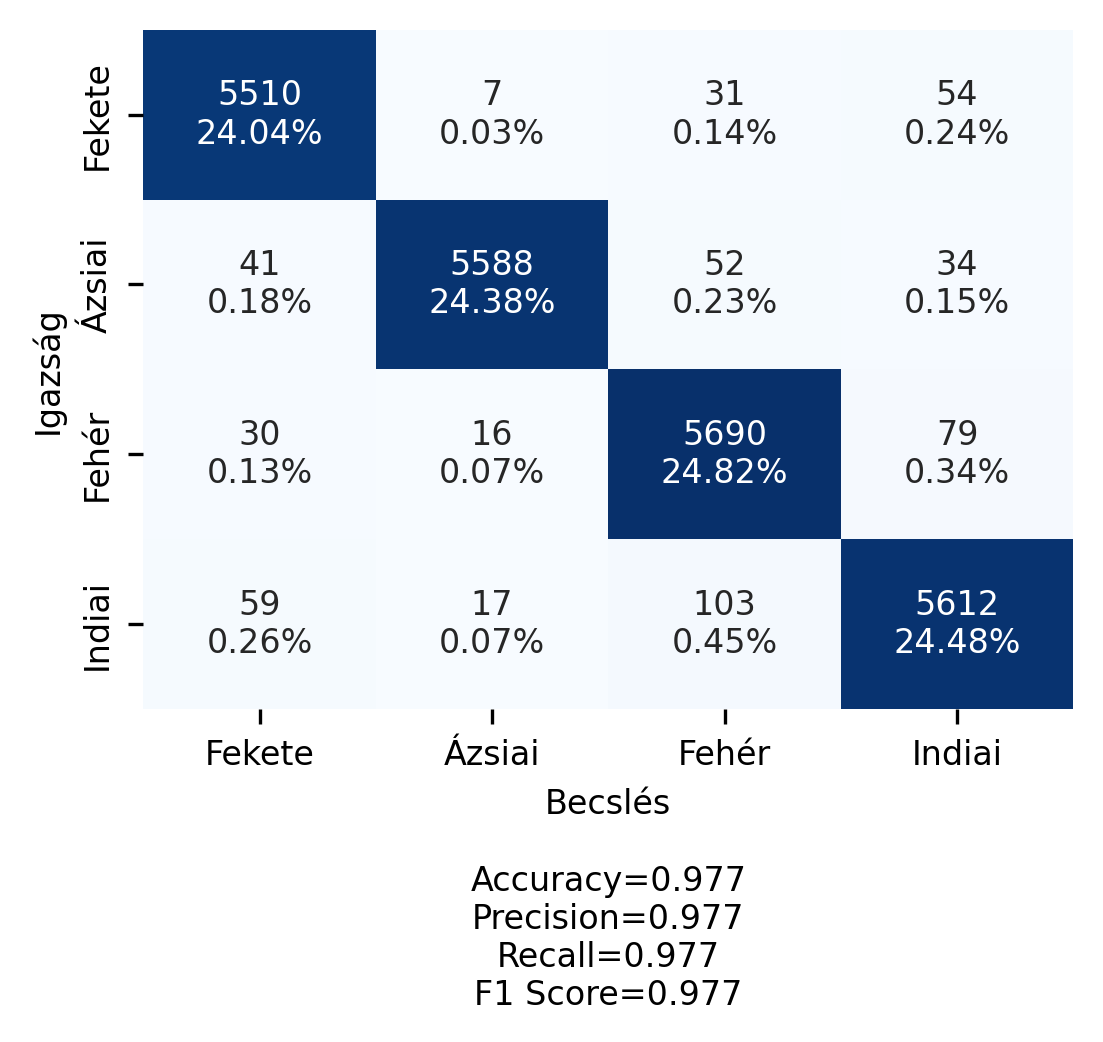
\includegraphics[width=0.7\columnwidth]{figures/conf_race.png}
	\caption{A rassz osztályozó modell igazságmátrixa és pontossági metrikái.}
	\label{fig:conf_race}
\end{figure}

\subsubsection*{Életkor becslése}
Az életkor osztályozó modell tanításához az IMDB-WIKI arclenyomat adathalmazt használtam. Mivel az adathalmazban pontosan szerepelnek az életkorok, először regressziós modellel próbálkoztam, de annak a pontossága nem lett túl jó ($R^2$ értéke 0,6 körüli volt). Ezt követően az életkorokat csoportosítottam 20 éves intervallumokon. Így négy életkor osztályt kaptam: 1-19 éves, 20-39 éves, 40-59 éves és 60 év fölöttiek csoportját. Ezzel a módszerrel már jobb eredményt értem el (ACC = 0,77), ami továbbra sem olyan jó, mint amit a korábbi modelleknél sikerült elérnem. Ez belátható annak, hogy az adathalmazban főleg fiatal - középkorú felnőttek vannak (lásd: \ref{fig:agedist}. ábra). A 20 év alattiak és 60 év fölöttiek aránya elég kicsi. A modell jóságát az alábbi \ref{fig:conf_age}. ábra mutatja.

\begin{figure}[ht]
	\centering
	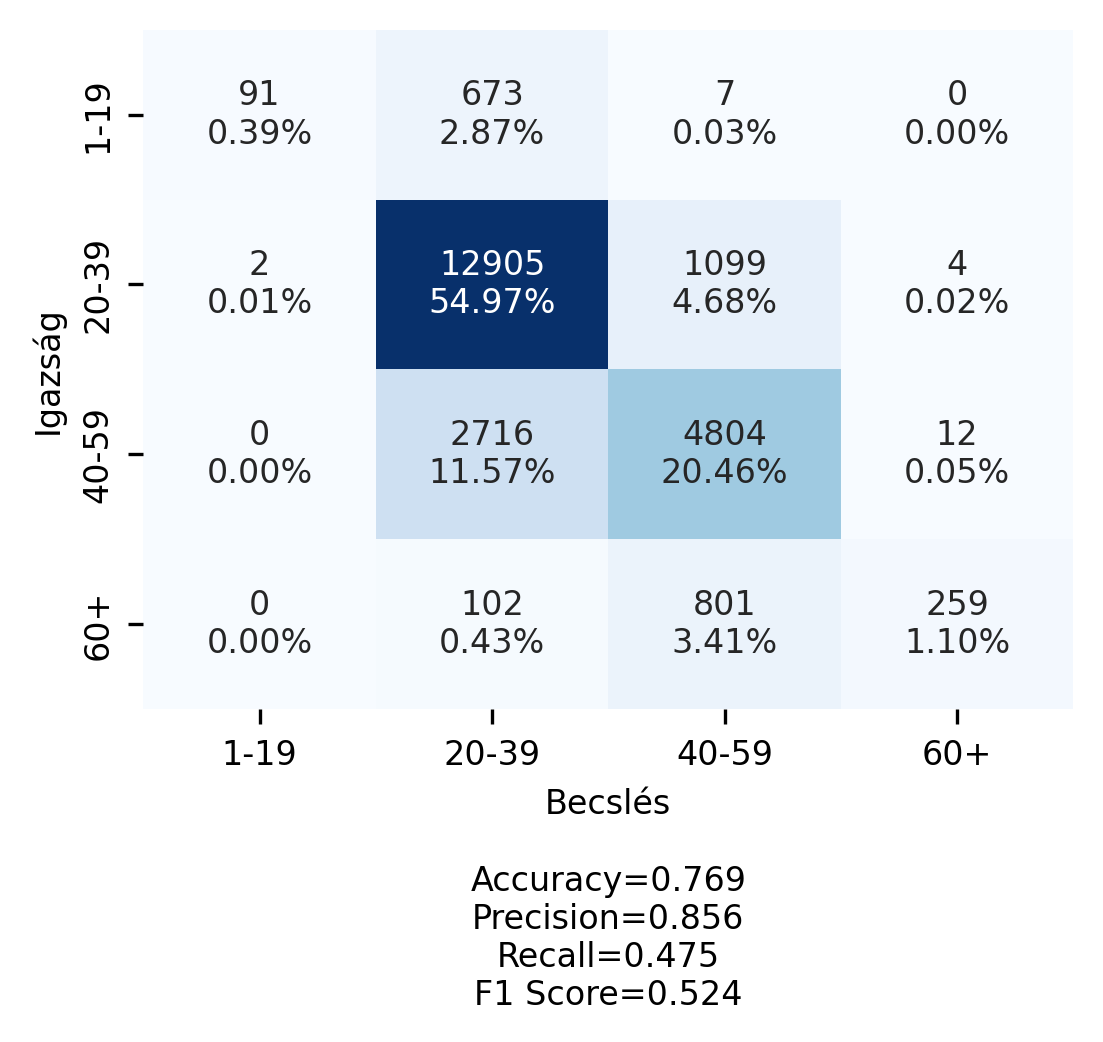
\includegraphics[width=0.7\columnwidth]{figures/conf_age.png}
	\caption{Az életkor osztályozó modell igazságmátrixa és pontossági metrikái.}
	\label{fig:conf_age}
\end{figure}

\subsubsection*{Identifikációs modell}

Az identifikációs modell képes megbecsülni a bemeneti arclenyomat alapján, hogy az melyik személyhez (ID-hoz) tartozik. Erre a feladatra a korábbiaktól eltérően nem gépi tanulási modellt alkalmaztam, hanem távolságmérés alapján határoztam meg a legvalószínűbb személyt. A modellnek szüksége van arclenyomat vektorokra, és hozzájuk tartozó címkékre. Ez alapján az egyes címkékhez tartozó arclenyomatok átlagát számítja ki (amik a centroidok). Új minta becsléséhez a centroidoktól vett távolság alapján találja meg azt az ID-t ami legvalószínűbb találat. A modell működését a \ref{lst:idmodel}. kódrészlet mutatja be.

\begin{lstlisting}[language=python, caption=Az identifikációs modell működése., label=lst:idmodel]
class IDModel:
	def __init__(self, embeddings, ids):
		'''
		embeddings : [np.ndarray] Nx128 - tanito mintak (arclenyomatok)
		ids : [np.ndarray] Nx1 - mintakhoz tartozo azonosito cimkek (pl: 'id00001')
		'''
		self.embeddings = embeddings
		self.ids = ids
		self.unique_ids = np.unique(ids)
		self.centroids = np.zeros((self.unique_ids.shape[0], embeddings.shape[1]))
		for i in range(len(self.unique_ids)):
			id = self.unique_ids[i]
			idx = np.where(ids == id)[0]
			centroid = np.mean(embeddings[idx], axis=0)
			self.centroids[i] = centroid

	def predict(self, new_embeddings):
		# adott arclenyomat es a centroidok tavolsagok osszevetese
		y_hat = np.zeros(len(new_embeddings)).astype('object')
		for i in range(len(new_embeddings)):
			d = np.linalg.norm(new_embeddings[i] - self.centroids, axis=1, ord=2)
			d_min_idx = np.argmin(d)
			y_hat[i] = self.unique_ids[d_min_idx]
		return y_hat

	def score(self, X_test, y_test):
		# becsles pontossaga
		y_hat = self.predict(X_test)
		return np.sum(y_hat == y_test) / len(y_test)
\end{lstlisting}

Összegezve, a három demográfiai adat közül a nemet és a rasszt nagy pontossággal lehet becsülni, míg az életkor becslése nehezebb feladat. Jobb eredmény érhető el akkor, ha kiegyensúlyozottabb életkor arckép adathalmazból indulunk ki. Tekintve, hogy én csak publikusan és ingyenesen elérhető arckép adathalmazokat vizsgáltam, egy valós támadó ennél jobb pontosságot is elérhet, így az eredményem egy alsó becslésnek tekinthető. Az identifikációs modellel is jó pontosságot sikerült elérni, csak néhány esetben adott téves becslést. A négy modell eredményeit a \ref{tab:pontossagok}. táblázat foglalja össze.

\begin{table}[ht]
	\centering
	\begin{tabular}{|c|c|c|c|c|}
		\hline
		& ACC & PREC & REC & F1  \\
		\hline
		\hline
		Nem & 0.988 & 0.987 & 0.989 & 0.988 \\
		\hline
		Rassz & 0.977 & 0.977 & 0.977 & 0.977 \\
		\hline
		Életkor & 0.769 & 0.856 & 0.475 & 0.524 \\
		\hline
		ID & 0.998 & 0.998 & 0.998 & 0.997 \\
		\hline
	\end{tabular}
	\caption{Az osztályozó modellek pontossága}
	\label{tab:pontossagok}
\end{table}
 
%--------------------------------------------------------------------------------------------------
\subsection{Adatvédelmi elemzés}  % (1-2 oldal)
\label{sec:adatvedelmi_elemz}


% TODO

% - Adatvédelmi elemzés -> milyen riskek vannak (munkacsoport szerint) pl: több info kiderülése 1 emberről probléma, adatszivárgás: le tudja szűkíteni, hogy ki lehet az, singling out, vagy lehet arcot rekonstruálni az embeddingből, újraazonosítás.

% Be lett mutatva, hogy a támadó kinyerheti az adatokat
% ez milyen kockázatokkal jár? Mire tudja felhasználni?



%--------------------------------------------------------------------------------------------------